\documentclass[12pt]{article}
\usepackage[a4paper, total={6in, 8.5in}]{geometry}
\usepackage{graphicx}
\graphicspath{ {images/output/} }
\usepackage{amsmath}
\usepackage{minted}
\usepackage{multicol}
\usepackage{caption}
\usepackage[english]{babel}
\usepackage{placeins}
\usepackage{titling}

\title{Basic documentation using mark down}
\author{}
\date{}

\begin{document}
\pagenumbering{gobble}
\vspace*{\fill}
\begin{center}

    \emph{Heaven's Light is Our Guide} \\
    \textbf{Rajshahi University of Engineering and Technology} \\

    \begin{figure}[H]
        \centering
        
\includegraphics[scale=.34]{images/RUET_logo.png}
        \label{fig:ruet_logo}
    \end{figure}
    \vspace{5mm}

    \textbf{Course Code}\\
    ECE 3118\\
    \vspace{3mm}
    \textbf{Course Title}\\
    Software Engineering \& Information System Design Sessional

    \vspace{5mm}

    \vspace{5mm}
    \textbf{Lab Report 1: Basic documentation using mark down.}

    \vspace{15mm}

    \begin{tabular}{c|c}
        \textbf{Submitted to} & \textbf{Submitted by} \\
        Oishi Jyoti           & Md. Tajim An Noor     \\
        Assistant Professor   & Roll: 2010025         \\
        Dept of ECE, Ruet     &                       \\
    \end{tabular}

\end{center}
\vspace*{\fill}


\maketitle
\section*{Introduction}
Markdown is a lightweight markup language designed by John Gruber in 2004 to simplify text formatting using plain syntax. It allows users to add headers, lists, links, images, and more without complex software, making Markdown files readable even without rendering, which is ideal for documentation and technical writing.

Markdown is part of a larger group of markup languages, including HTML, XML, and LaTeX, which structure content with specific symbols or tags. Unlike HTML, which uses tags like <p> for paragraphs, Markdown uses symbols like \# for headers and * for lists, enabling quick formatting while remaining user-friendly and versatile for content creation.

\section*{Code}
\begin{multicols}{2}{|}
    \begin{minted}[linenos,breaklines,breakanywhere]{markdown}
### Types of header

# Header 1

## Header 2

### Header 3

#### Header 4

##### Header 5

###### Header 6

### Emphasis

_This is italic writing_<br>

**This is bold writing**<br>

**_This is bold-italic writing_**<br>

### Strike through

~~A line through the text~~<br>

### Links

https://github.com/ <br>

https://www.google.com/ <br>

### Masked Links

[Google](https://www.google.com/) <br>

[Github](https://github.com/)

### Table

| Dept Name | Dept Code | Students per year |
| --------- | --------- | ----------------- |
| ECE       | 10        | 60                |
| CSE       | 03        | 180               |
| EEE       | 01        | 180               |

### image

![Landscape](https://wallpapers.com/images/high/genshin-impact-fantasy-sunset-scenery-i3v1rmx41gnu0cv7.webp)

### Source Code:

```python
def display_message():
    print("HELLO WORLD.")

# Call the function
display_message()
```    
\end{minted}
\end{multicols}

\section*{Output}

\begin{figure}[hbt!]
    \centering
    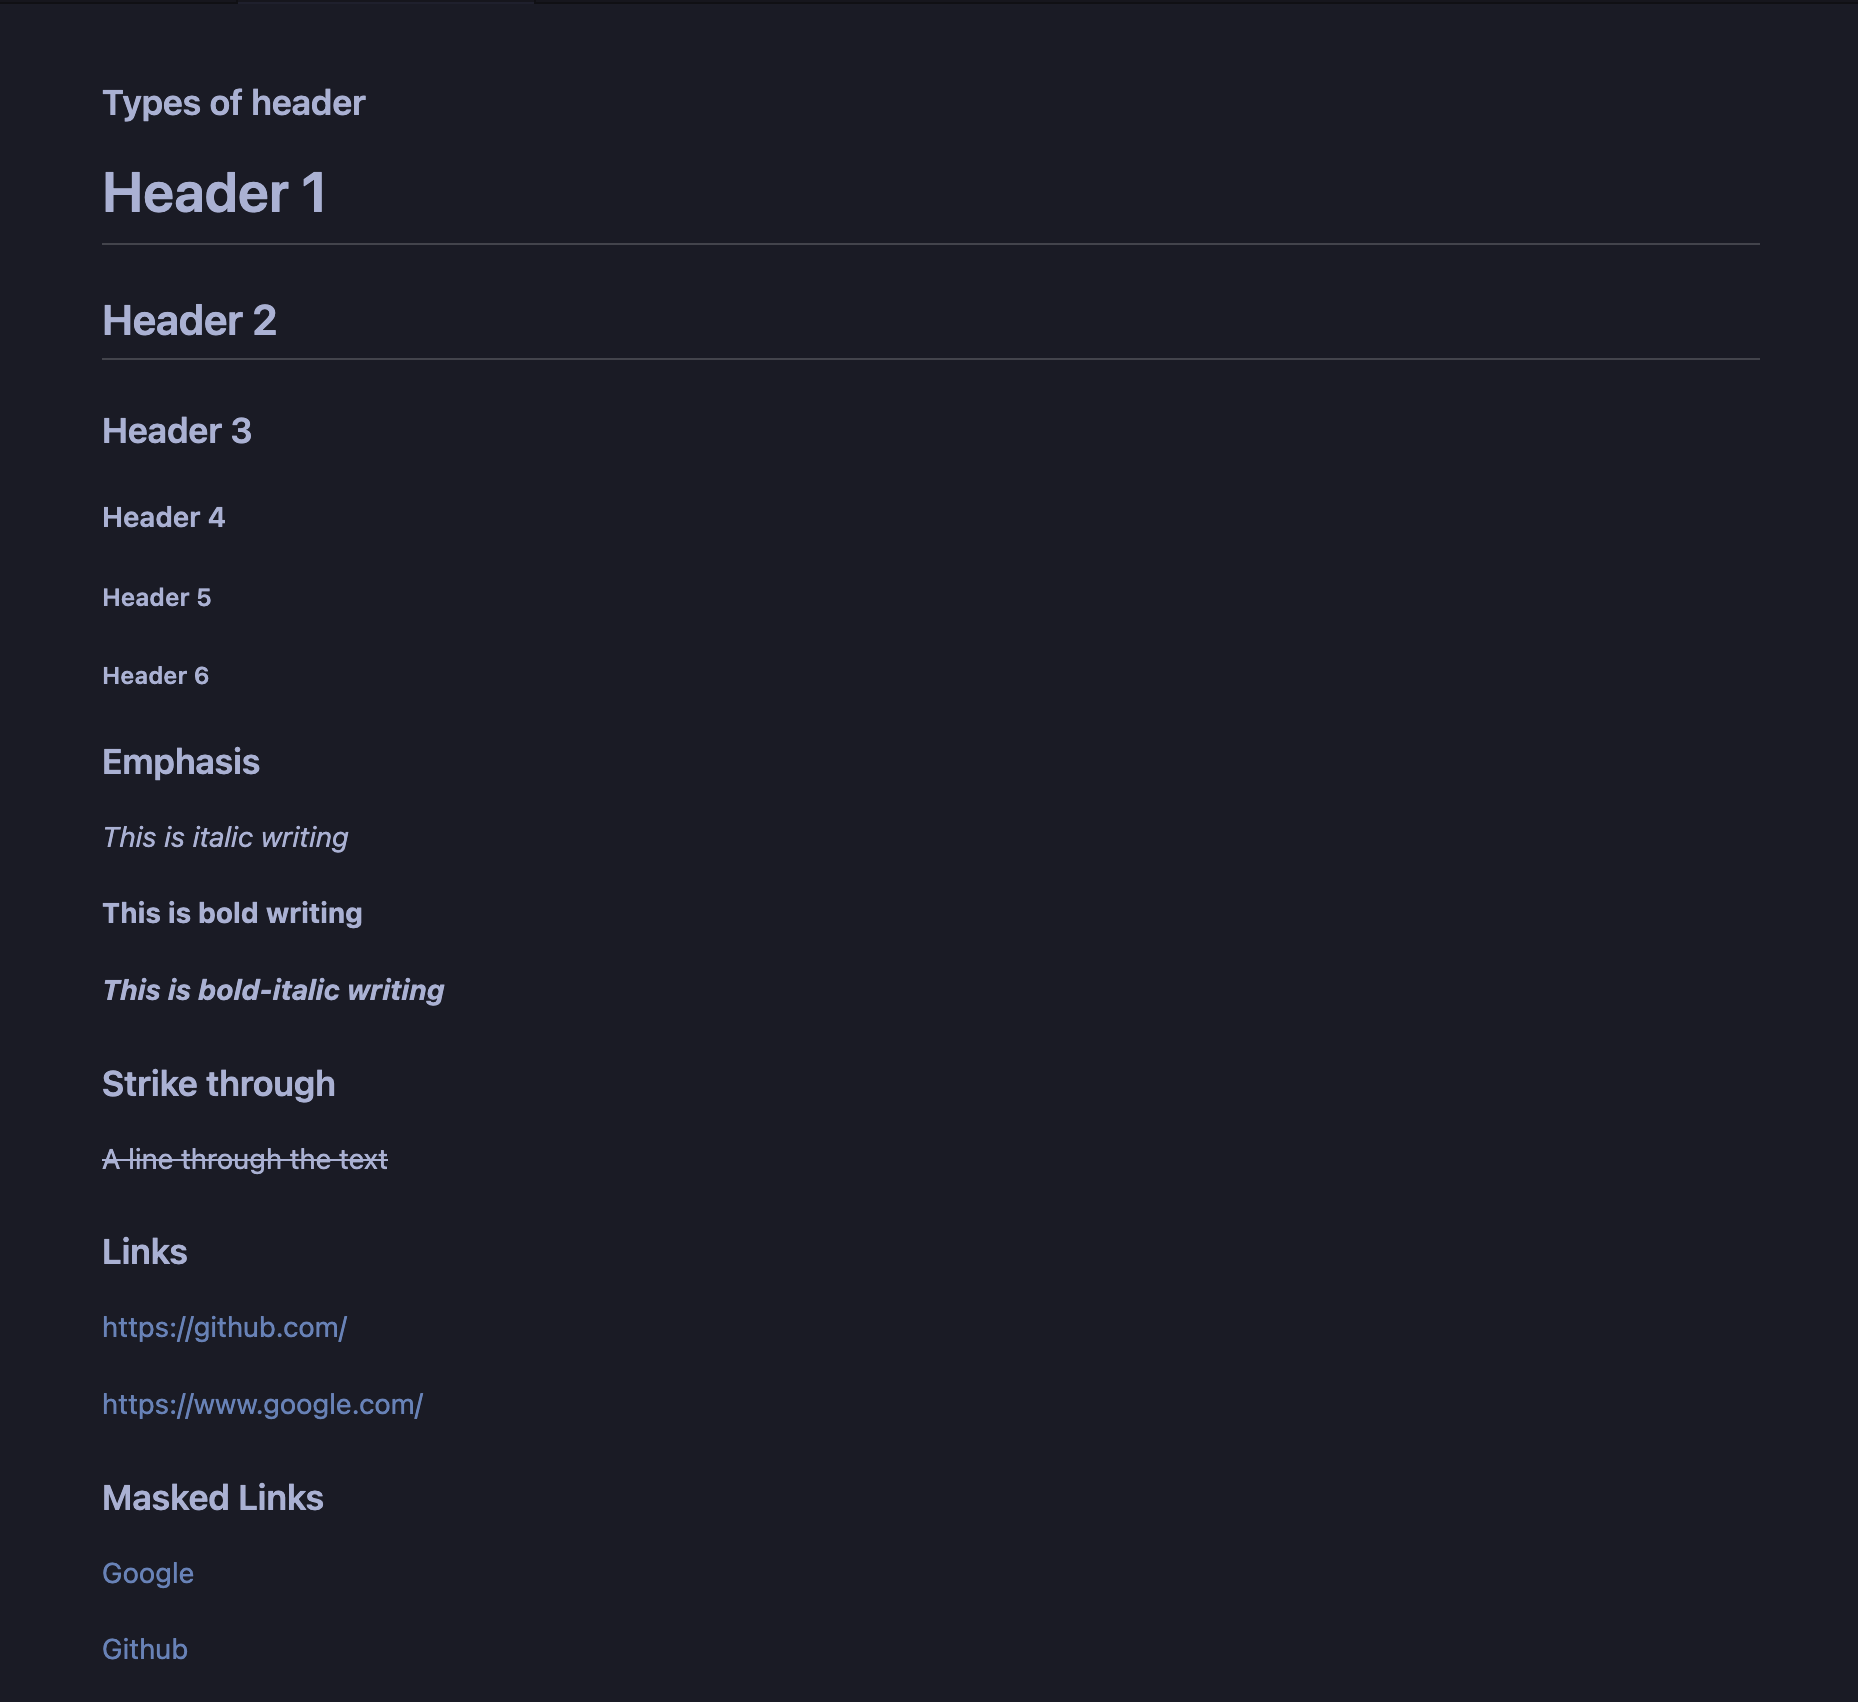
\includegraphics[width = .6\textwidth]{md1.png}
\end{figure}

\begin{figure}[hbt!]
    \centering
    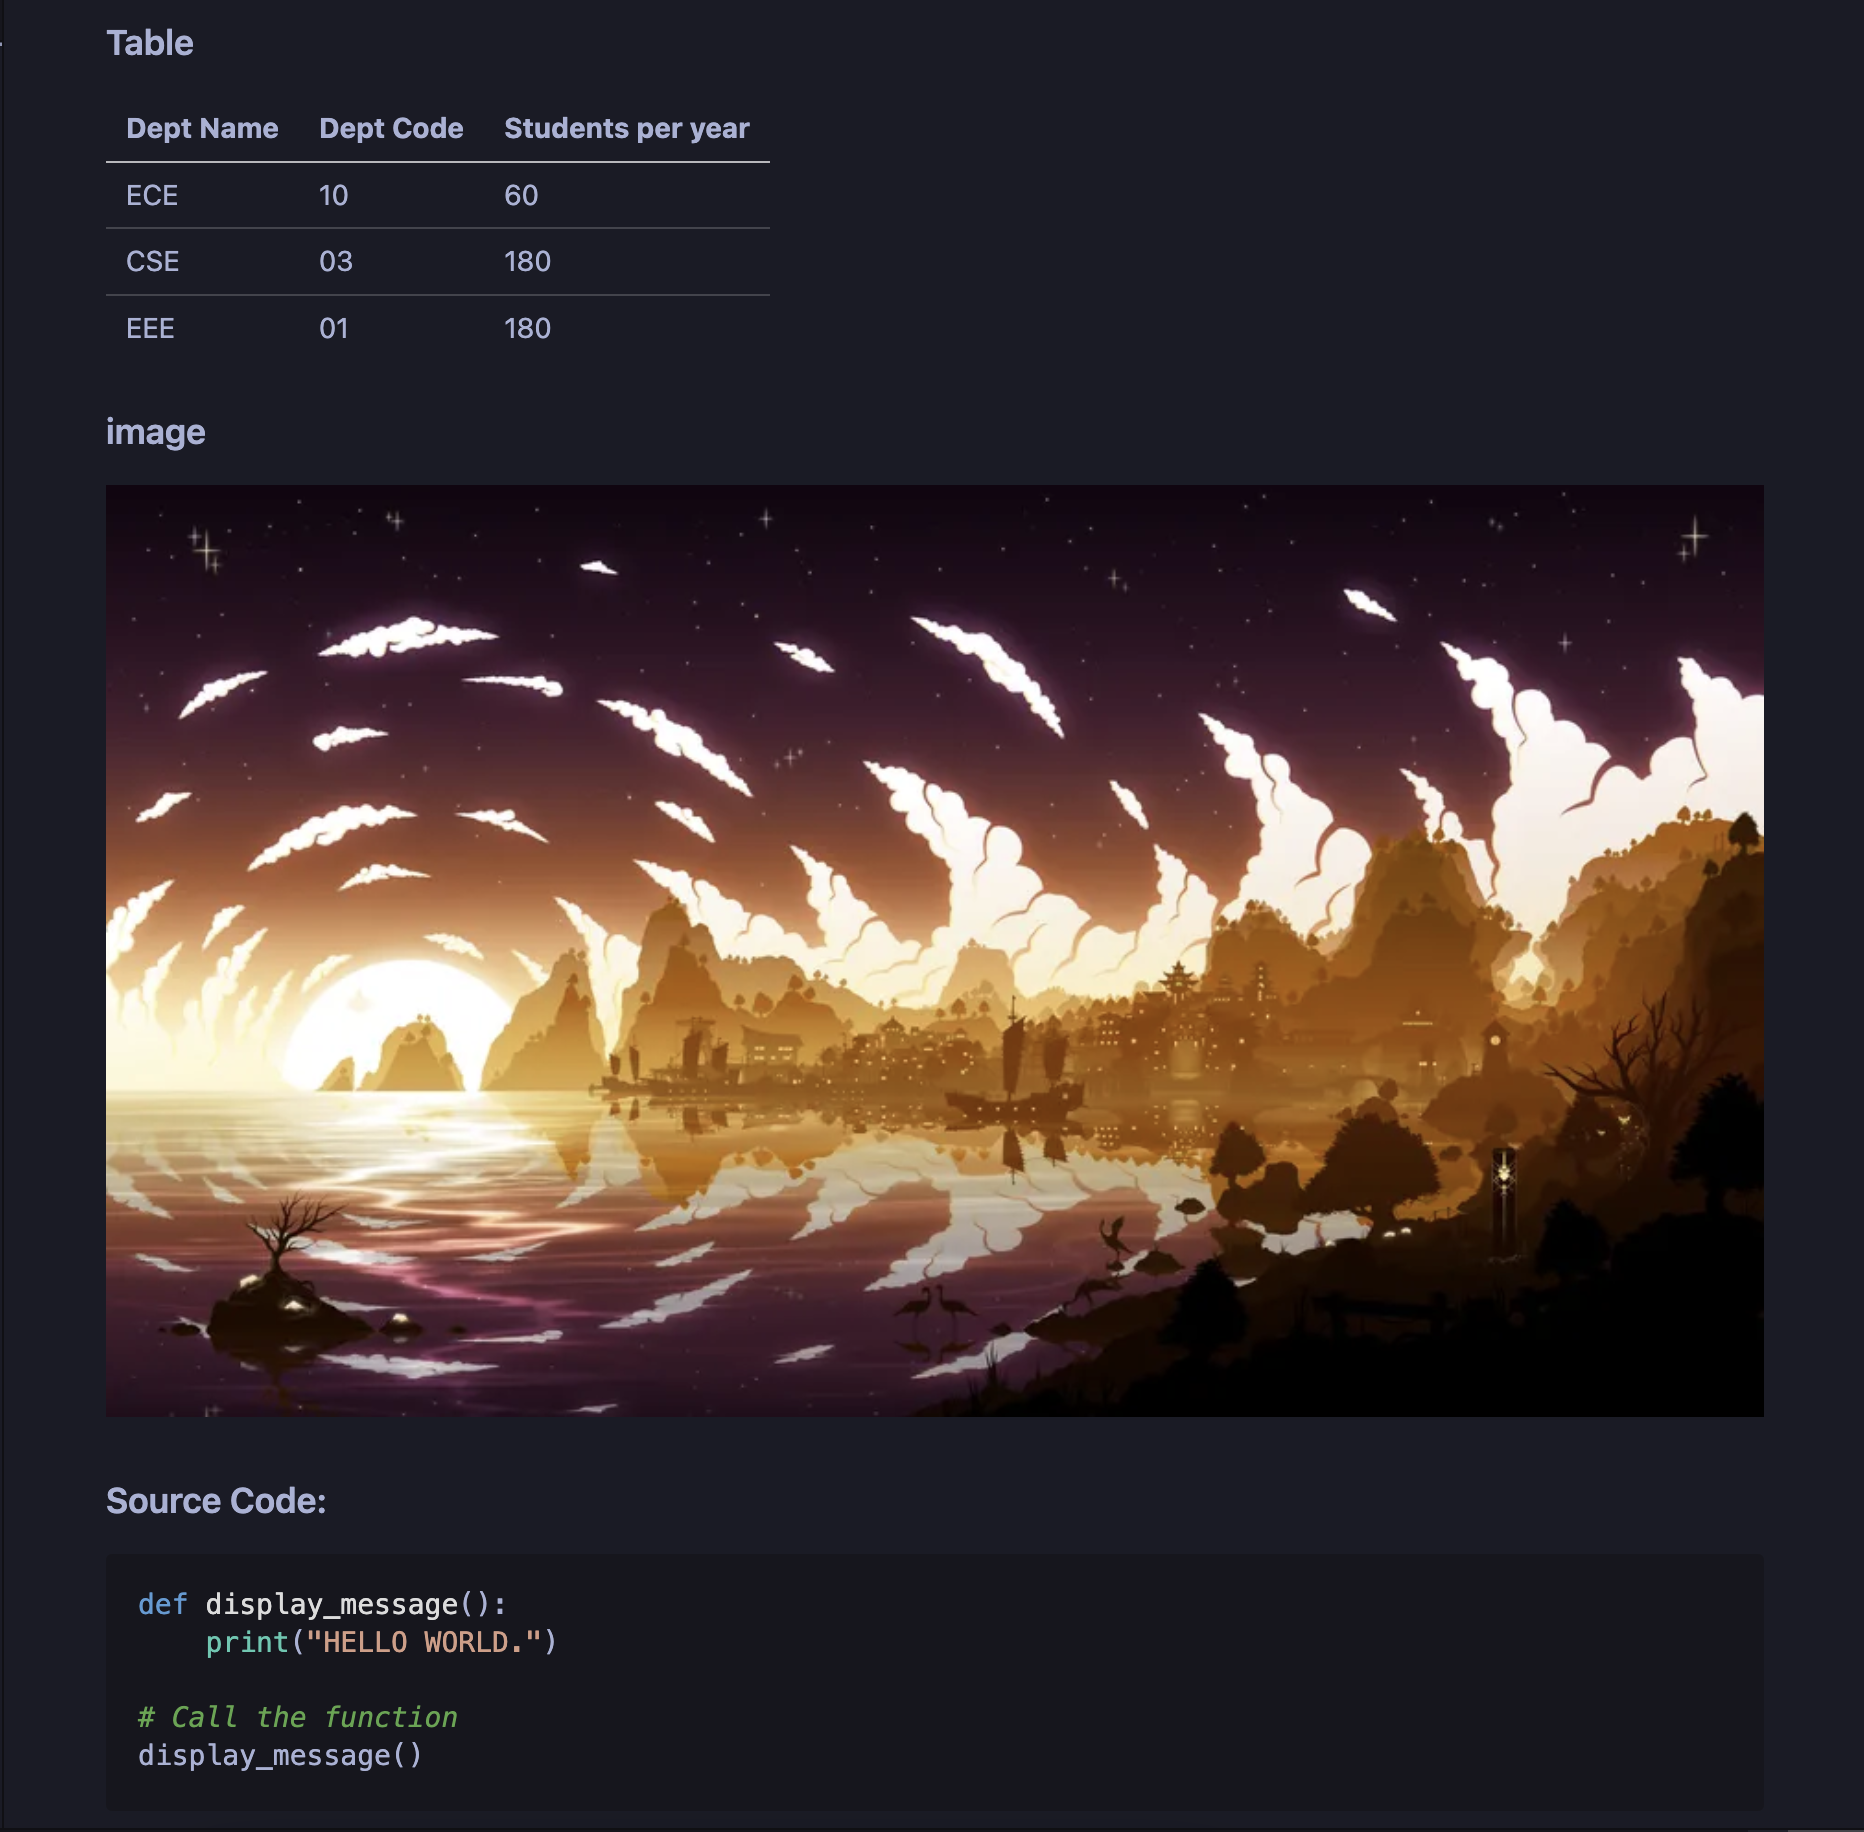
\includegraphics[width = .6\textwidth]{md2.png}
\end{figure}

% \bibliographystyle{IEEEtran}
% \bibliography{ref}



\end{document}
